\documentclass[a4paper, 11pt]{article}
\usepackage[top = 1.1in, bottom = 1.1in, left = 0.6in, right = 0.6in]{geometry}
\usepackage{amsmath}
\usepackage{graphics}
\usepackage{graphicx}
\usepackage{subcaption}
\usepackage{caption}
\usepackage{listings}
\usepackage{multirow}
\usepackage{multicol}
\usepackage{url}
\usepackage[export]{adjustbox}
\usepackage[labelfont=bf]{caption}

\usepackage{lipsum}
\newenvironment{Figure}
  {\par\medskip\noindent\minipage{\linewidth}}
  {\endminipage\par\medskip}

\begin{document}
%%Title
\Large
\begin{center}
\hrulefill \\
\textbf{IMAGE PROCESSING} \\
SF2 - SECOND INTERIM REPORT \\
\vspace{0.2cm}
\normalsize 
Quang-Thinh Ha - CRSid: qth20 \\
\hrulefill \\
\end{center}

\normalsize

\section{Introduction}
This is a follow-up for the first-interim report of Image Processing project. Particularly, this report will focus on exploring three different energy compaction schemes, \textit{Discrete Cosine Transform}, \textit{Lapped Bi-Orthogonal Transform} and \textit{Discrete Wavelet Transform}. The report will conclude with a final comparison between all the schemes that have been investigated so far. 

\section{Discrete Cosine Transform}
Discrete Cosine Transform (DCT) is a technique for converting a signal into elementary frequency components. It has been widely used in image compression. 

In one-dimensional form, each element of the transformed list is the inner product of the input signal and a \textit{basic vector}. A graph containing 8 basic vectors is included in Figure 1. Since the basis functions are orthogonal (and also orthonormal from normalisation), the coefficients are uncorrelated to each other and missing one coefficient does not affect the remaining ones. This provides a reliable reconstruction even if one or more coefficients are missing. Therefore, DCT is surprisingly good for compression. 

For the purpose of this project, since the input signal is two-dimensional - an \textit{image}, we need a 2D version of DCT. For a general matrix $n \times m$ matrix, the 2D DCT is constructed in a simple way: the 1D applied to each row and column of the result. In this case, the two-dimensional basis matrix is the outer product of two of the 1D basis vectors. Examining Figure 2 will give a better understanding of the statement. 

Applying a 2D DCT, followed by grouping each coefficient type into a small sub-image will provide Figure 3. An observation is made that as frequencies increase, (moving toward the sub-image at the bottom-right), less elements of the original image - which is presented at the top-left corner - is included in the sub-images. This means that the energies of the sub-images decrease as we move toward the bottom right corner.

After testing out various transform sizes, along with their corresponding visual effects, a list of reconstruct images, using inverse DCT based on different transform size, and a graph showing their compress ratio are presented in Figure 4 and 5 respectively. 

In Figure 4, it is noticeably that there are obvious artefacts when using larger transform sizes. The most vivid area is where the edges are. Since DCT is actually applied \textit{block by block}, this might not be the best approach as \textit{blocks do not take edges and texture into consideration}. 

In general, DCT will throw away very high frequency components (including edges), and this explains why it might \textit{not} be a good idea to apply DCT for images with a \textit{great number of high frequency components}. Clear examples include pictures containing rich texture, transitions and sharp edges. 

A look at Figure 5 concludes that, the optimal choice when consider the balance between compress ratio and image quality is \textit{using a transform size of $8\times8$}, which gives a \textit{compress ratio} of \textbf{2.9501}.

In terms of entropy, summing the total bits calculated from each individual sub-image result in a \textit{smaller} than the value obtained from generating total of bits from the whole big image. This is because when combining information from each sub-image into one big one, more information is needed, resulting in higher entropy. By just considering the amount of information for each sub-image and sum the total entropy at the end, the obtained value should be lower. 

If entropy is calculated independently for each pixel, i.e. calling \textbf{dctbpp(Yr, 256)} regardless of transform sizes, the value of entropy received should be 0. This is because each pixel is determined with an allocated pixel, giving $\mathtt{p = 1}$ and $\mathtt{log(1) = 0}$. This means that the image contains `zero' information. As this cannot be right, this result is not practical.

\section{The Lapped Bi-orthogonal Transform (LBT)}
One of the most obvious artefacts coming from DCT is the \textit{blocking effect}. Since DCT separate images into parts/blocks, artificial discontinuity between adjacent block is inevitable (Figure 4). One of the solution for this is to allow \textit{overlap} between blocks. This is done by applying a \textit{forward} and \textit{backward} filtering before and after the DCT\footnote{The pre-filtering is sometimes addressed as a \textit{Photo Overlap Transform}. Combining a POT and a DCT is equivalent to a particular type of LBT.}. LBTs allows a smoother decay of filter functions to 0 at their boundaries, and hence a reduction of the `block' artefact compared to DCT. 

Let's first look at the forward filter \textbf{Pf} and the backward filter \textbf{Pr} that is applied to the image prior and post DCT, which is quoted in Figure 6. The scaling factor, \textit{s}, represents the relative contributions of the forward and backward filter. $s = 1$ represents an equal contribution from both, while $s = 1.5$ means that the forward filter is weighted more significant compared to the backward one. As a result (Figure 7), there is more overlapping between blocks for the forward filter compared to the backward one. 

The next step is to find the scaling factor that gives the best compression ratio. Based on the result presented in Figure 10, for an $8 \times 8$ DCT, the \textit{optimal value for the scaling factor is \textbf{1.4018}}, giving a compress ratio of \textbf{3.0638}. Figure 8 shows the visual quality as the scaling factor increases from 1 to 2. As observed, when the scaling factor approaches 2, the sky becomes even `blockier'. This `blocky' artefact is due to the basis functions are now too long and overlap between blocks more. Consequently, the quantisation error is spread out more between blocks, resulting in more `pixelated' constructed image. 

One obvious artefact on all Figure 11 images are the `ringing' effect around the edges. There seems to be some `wiggling' area around the sharp edges of the lighthouse and the fences, and this does not seem to increase against the scaling factor. Yet further on, it is shown that changing the transform size of the DCT enhances this kind of artefact.

Following the same methodology for DCT, the next part is to look at the performance of LBTs using different transform sizes. One major point to address to the readers is that the total number of bits presented in Figure 9 is calculated by always using $16 \times 16$ blocks regardless of the transform size, which explains why the trend line is different from the one shown in Figure 8 for DCT. When using the same calculation between two methods, it is obvious that the peak compression ratio for LBT is higher that the same obtained value for DCT (\textbf{3.3539} vs \textbf{3.2251}). This is expected, thanks to the overlapping parts of the basis functions between blocks. The number of transform coefficients is now equal to the block size, and hence cause a reduction in the total number of bits required to encode the image.

Along with this slight rise in compress ratio, as mentioned before, the block artefact is now suppressed. However, the graph follows interesting trend as the transform size increases. Using any larger transform size results in a worse performance of LBT compared to DCT. 

This is further confirmed by looking at the result image obtained from LBTs in Figure 11. In the case of using $64 \times 64$ transform size, the `ringing' artefact around sharp edges becomes even more obvious. Another interesting detail is marked in red box. There seems to be a `shadow' edges represent in the sky. This may means that some edges get overlap and represented in the area that there should not be any. Simply speaking, it is as there is a mirror between block boundaries but for the case of larger transform size, the reflected image becomes more obvious and cause a significant artefact for the constructed result. 

\section{Discrete Wavelet Transform}
The final method of energy compaction that is investigated in this report is the \textit{Discrete Wavelet Transform.}

Wavelets are signals which are local in time and scale and generally have an irregular shape. A wavelet transform can be used to decompose the a signal into component wavelets\footnote{For further details, please refer to the lab handout.}.

In terms of images (where signals are 2D), the result of the complete DWT\footnote{The DWT technique presented in this report is \textit{binary wavelet tree.}} is a set of four sub-images: the blurred version of the original image, in which the high frequency components are represented in three other sub-images. These components correspond to the vertical, horizontal and diagonal differences - or simply \textit{edges} - between the original image and the blurred one. Figure 13 represents a result of one DWT iteration on the image. 

Let's look at DWT performance on image compression by examining the compression ratio on two different images, using two different schemes on Figure 14. The optimal choice for both images is to use 5-iteration DWT, which provides a compress ratio of \textbf{3.1023} and \textbf{1.9188} for the Lighthouse and the Bridge images, respectively. Using constant quantiser only provides an optimal compress ratio of \textbf{2.7744} and \textbf{1.8063}. Hence, it is concluded that \textit{equal MSE}, with more iteration, provides better compress ratio and visual quality. Based on Figure 15, the picture get less `pixelated' when a 5-iteration DWT is used instead of one level. The reason that DWT performs better on the Lighthouse image compared to the Bridge is due to the features on each image. Lighthouse contains a large number of vivid edges in horizontal, vertical and diagonal directions, whereas these edges are in more ambiguous orientations for the Bridge image because of the bushes. That is why the bottom right sub-image (where the diagonal edges are extracted) in Figure 13 barely shows anything. This results in a worse performance of DWT, which can be rectified if \textit{complex DWT} is used instead. Complex DWT accounts for edges along different orientations. 

In order to obtained the correct ratio between quantise steps for each sub-images in the \textit{equal MSE scheme}, the same technique that was used to achieve the similar ratio for \textit{Laplacian pyramid} is applied, but this time an impulse is placed in each sub-image separately. To avoid edge effects, the impulse needs to be placed away from the edge of the sub-image, which is why result iterations of more than 5 (producing a final blurred image of size $4 \times 4$) is not presented here, due to finite size of the pixel.

There is one minor detail regarding how to achieve the ratio between quantisation steps of each sub-image. Each sub-image is treated as another `step' or iteration of DWT compared to the blurred image in the far left corner. In other words, energy of the constructed image contributed by the impulse from one sub-image is accepted to be inversely proportional to the corresponding quantise step, regardless of what iteration that sub-image belongs to. This, although provides relatively good result, contradicts the relationship between energy and quantise step. Three sub-images, even though each contributes energy to the final image differently, is still on the same level of iteration, and hence another relationship between their quantise steps and energy should be derived instead. Note also, it is obversed that the ratios between these three sub-images are not constant over iterations, which can make things more complicated.


Figure 16 shows that the objective differences between equal MSE and constant quantiser scheme is pretty much unrecognisable. There are tiny changes in lighting and position of shadowing when displaying one picture after another, but it is impossible to represent such details. Hence, the only factor that favours equal MSE is their better compression ratio. 

\section{Conclusion}
To sum up, the optimal choices of compression ratio so far for the Lighthouse image is approximately \textbf{3.3539} using LBTs with a transform size of $8 \times 8$. However, DWT also follows closely with \textbf{3.1023}, so it is quite debatable which one truly performs better. Bear in minds that so far all the results obtained are image specific, more investigation on other cases should be looked into. A full summary of the properties of the investigated scheme is presented in Table 1 of the Appendix. 

One tiny area that has been overlooked in the project so far is the \textit{computation time} when using more iteration. In the scale of this project, such thing will not become a determining factor, but this could be otherwise when image's size is scaled up significantly.

\newpage
\section*{APPENDIX}
\begin{multicols}{2}

\begin{Figure}
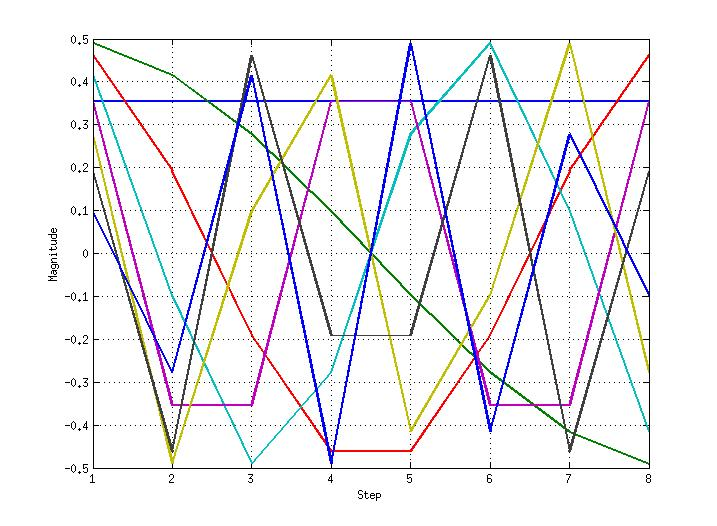
\includegraphics[width=0.8\linewidth, center]{dct_8.jpg}
\captionof{figure}{\small{\textbf{Basis vectors for DCT of length 8.} The constant factors are chosen so that the basis vectors are orthogonal and normalised. The DCT can then be written as the product of a vector and the \textit{n $\times$ n} orthogonal matrix whose rows are the basis vectors.}}
\end{Figure}

\begin{Figure}
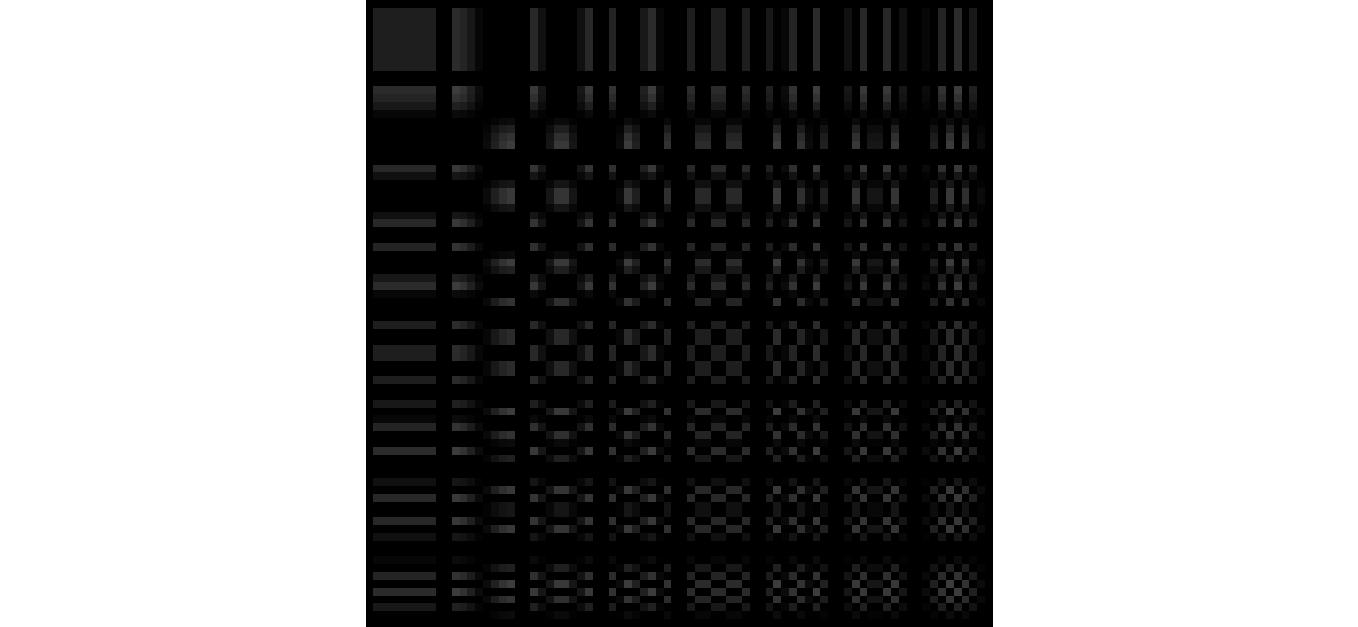
\includegraphics[scale=0.23, center]{dct_bases.jpg}
\captionof{figure}{\small{\textbf{Basis image for 2D DCT.} This image represents a 2D coefficients of DCT for 8 $\times$ 8 blocks of pixels. Each image represent a basis matrix which is characterise by a horizontal and a vertical spatial frequency. }}
\end{Figure}

\begin{Figure}
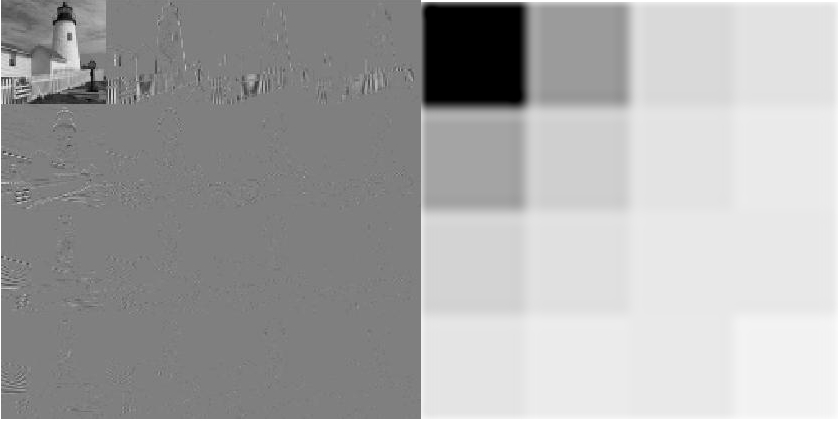
\includegraphics[width=1\linewidth, center]{dct_44_energy.jpg}
\captionof{figure}{\small{\textbf{2D DCT of the Lighthouse image and each sub-image corresponding energy.} Each sub-image is generated by first applying 2D DCT of 4x4 to the original image. This is then followed by grouping all the coefficients of a given basis matrix into a sub-image at a corresponding position. On the right, energy is plotted on the logarithmic scale and converted to intensity.}}
\end{Figure}

\begin{Figure}
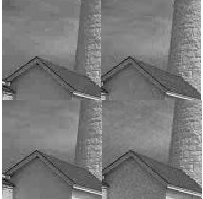
\includegraphics[width=1.0\linewidth, center]{dct_4_8_16_64_1.jpg}
\captionof{figure}{\small{\textbf{Reconstructed image using various transform sizes.} From left to right, top to bottom, the transform sizes are $4\times4, 16\times16, 8\times8 $ and $64\times64 $. Close examination around the edges of the pictures shows that the area near the edges becomes even `blockier' with larger transform size. This artefacts enhancement is a major drawback for the usage of DCT in image compression.}}
\end{Figure}

\begin{Figure}
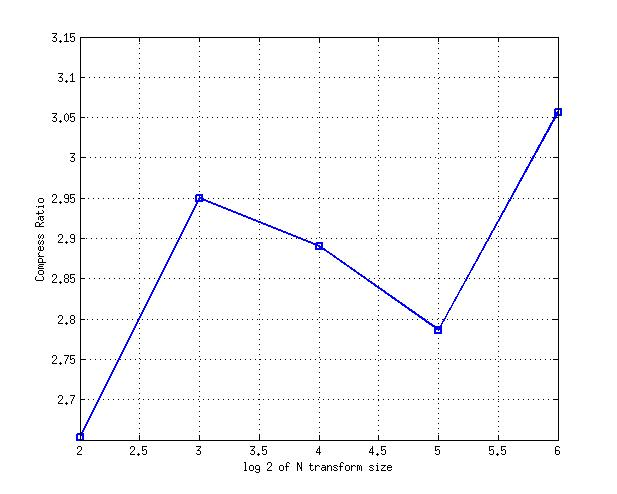
\includegraphics[width=1.0\linewidth, center]{dct_compress_ratio.jpg}
\captionof{figure}{\small{\textbf{Compress ratio when using different transform sizes.} Using larger transform sizes leads to the increase in compress ratio (another result, not included in the graph, using transform sizes of 128x128 will gives a compress ratio up to \textit{4.8736}. However, this increase comes with a cost of significantly reduced visual quality, as shown in Figure 4.}}
\end{Figure}

\end{multicols}

\newpage
\begin{multicols}{2}
\begin{Figure}
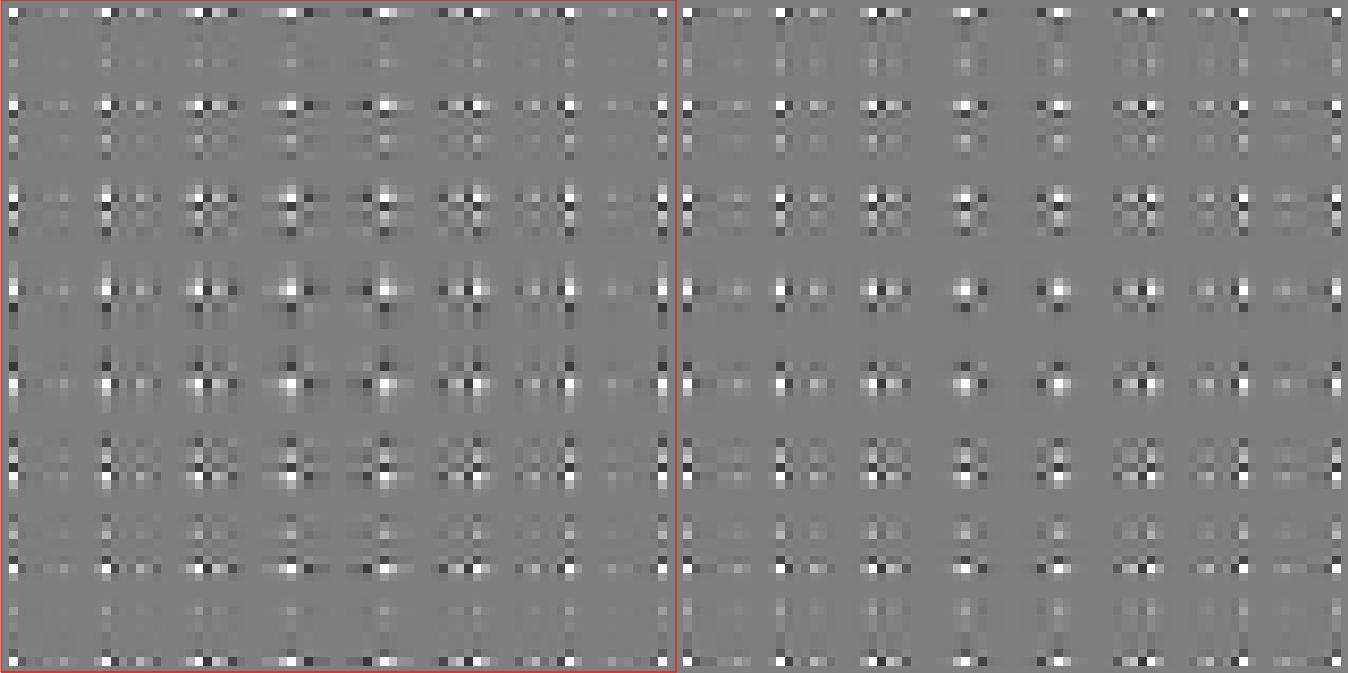
\includegraphics[width=1.0\linewidth, center]{lbt_bases_1_sqrt2.jpg}
\captionof{figure}{\small{\textbf{Bases for POT, with scaling factor of \texttt{1.5}.} On the left side, post-filter, there is less overlapping component compared to the picture on the right, which is the pre-filter. }}
\end{Figure}

\begin{Figure}
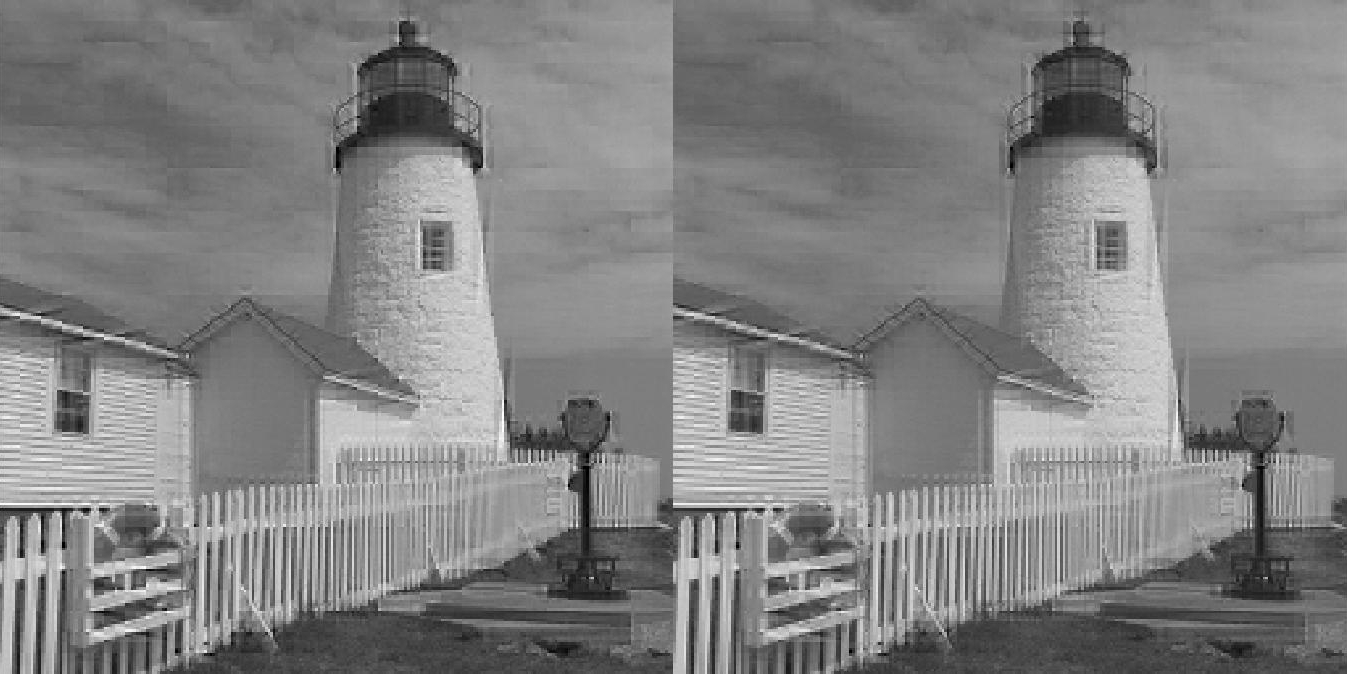
\includegraphics[width=1.0\linewidth, center]{lbt_xp_1_sqrt2.jpg}
\captionof{figure}{\small{\textbf{Effects of different pre-filter on the original image.} On the right, with higher scaling factor, the `wiggle' area on the image is more significant, representing more overlapping resulting image between blocks.}}
\end{Figure}

\begin{Figure}
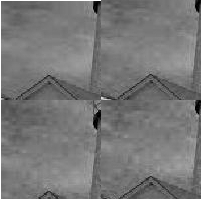
\includegraphics[width=1.0\linewidth, center]{lbt_visual_1_sqrt2_sqrt3_2_1.jpg}
\captionof{figure}{\small{\textbf{Effects of different scaling factor on the constructed image.} From left to right, top to bottom, the scaling factor values are 1; $\sqrt{2}$; $\sqrt{3}$ and 2. Moving toward the bottom right, the sky becomes even `blockier', arising from quantisation error.}}
\end{Figure}

\begin{multicols}{2}
\begin{Figure}
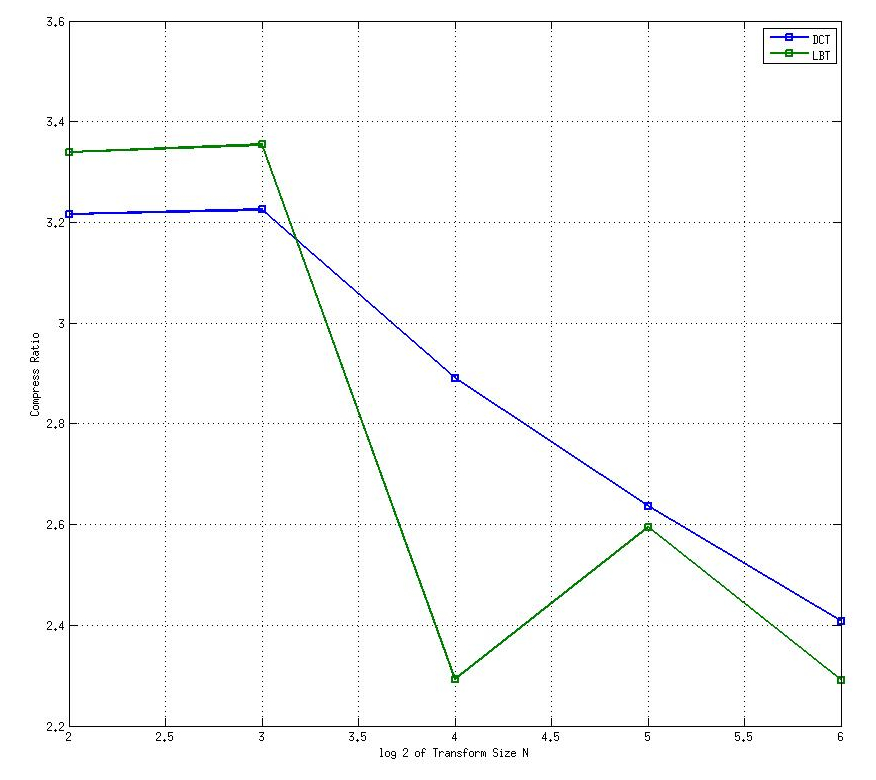
\includegraphics[scale=0.15, center]{compress_16_dct_lbt.jpg}
\captionof{figure}{\small{\textbf{Effects of using different transform sizes on compress ratio.} The peak value of LBT (green) and DCT (blue) is record at using a transform size of $8 \times 8$, with their corresponding compress ratio of \textit{3.3539} and \textit{3.2251}. The transform size is plotted in $\mathtt{log_{2}}$ base.}}
\end{Figure}
\begin{Figure}
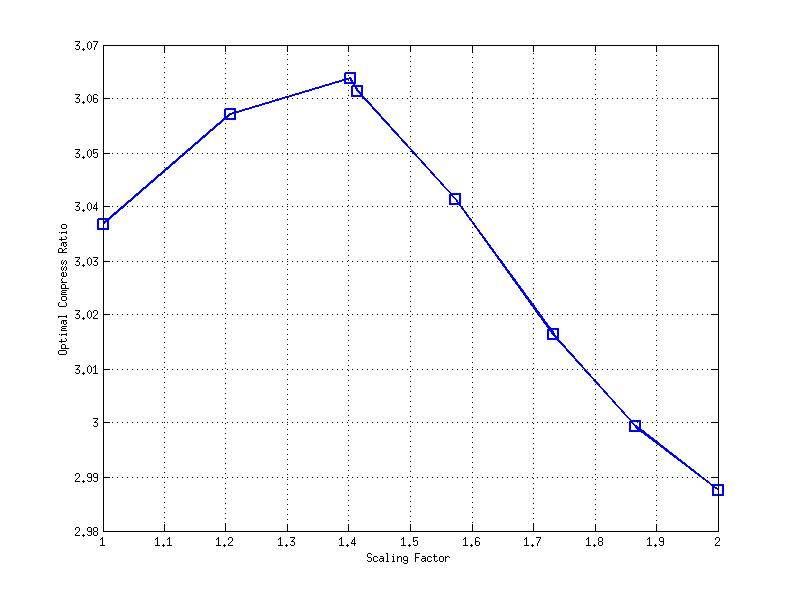
\includegraphics[scale=0.18, center]{lbt_8_scale_factor_compress_ratio.jpg}
\captionof{figure}{\small{\textbf{Variation of compression ratio against scaling factor}. The optimal value for the compression ratio of 3.0638 is a scaling factor of value 1.4018.}}
\end{Figure}
\end{multicols}

\begin{Figure}
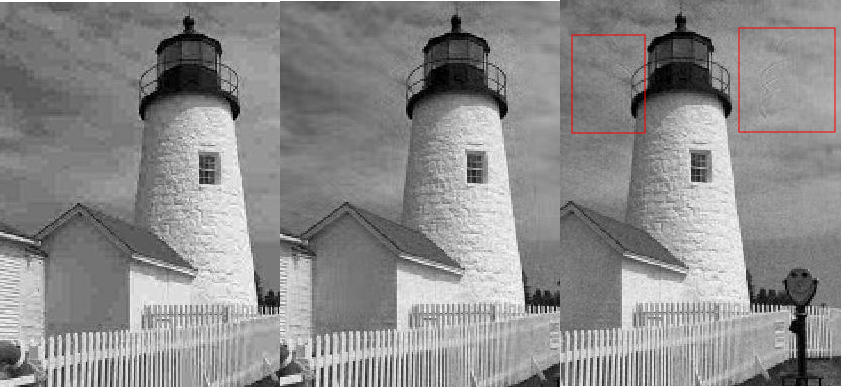
\includegraphics[width=1.0\linewidth, center]{lbt_4_16_64_1.jpg}
\captionof{figure}{\small{\textbf{Artefacts on the constructed image using transform sizes for LBTs.} From left to right, a transform size of $4 \times 4$, $16 \times 16$ and $64 \times 64$ is used. Note how the `ringing' effect around the edges becomes more obvious using larger transform size.}}
\end{Figure}

\begin{Figure}
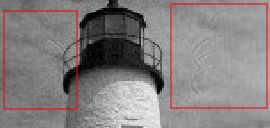
\includegraphics[width=1.0\linewidth, center]{lbt_64_close_up.jpg}
\captionof{figure}{\small{\textbf{Close-up zoom on the artefact of transform size $\mathbf{64 \times 64}$.} There seems to be a `shadow' reflection of the edge in the sky, around where the red box is drawn.}}
\end{Figure}
\end{multicols}

\newpage
\begin{multicols}{2}
\begin{Figure}
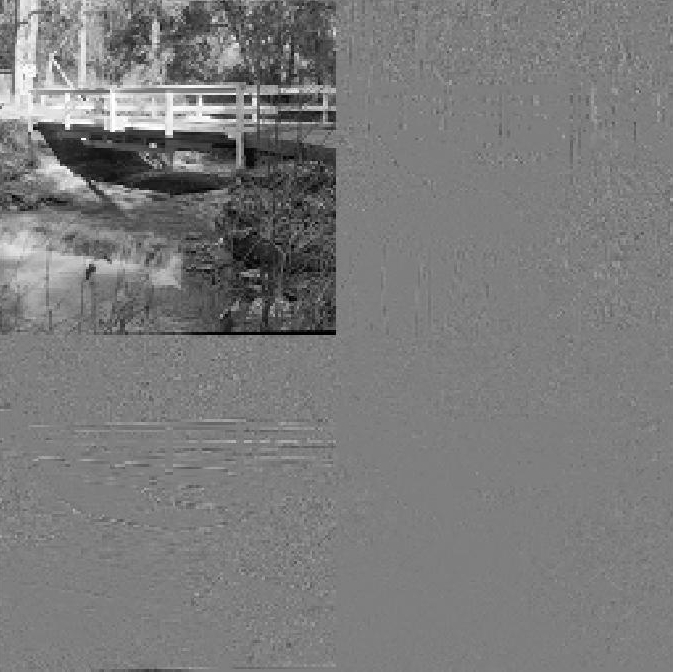
\includegraphics[width=0.8\linewidth, center]{b_y_dwt_1.jpg}
\captionof{figure}{\small{\textbf{Result from one iteration of DWT.} On the far left corner, the blurred version of the image is presented, where the other three contains the vertical, horizontal and diagonal edges of the original image.}}
\end{Figure}

\begin{Figure}
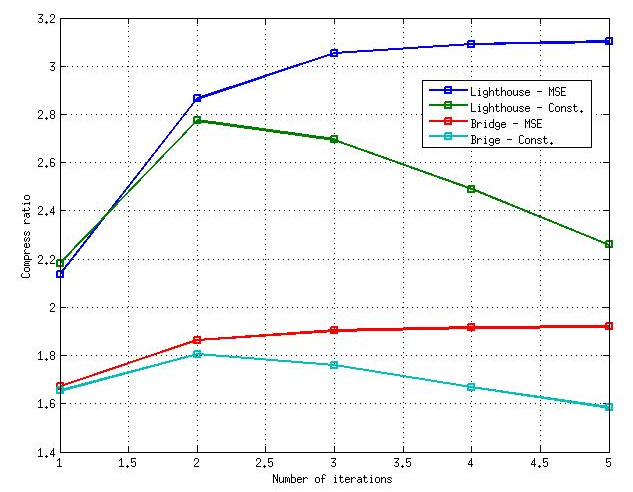
\includegraphics[width=1.0\linewidth, center]{dwt_ratio.jpg}
\captionof{figure}{\small{\textbf{Compress ratio obtained from applying two different schemes on two different images.} Overall, the equal MSE scheme outperforms the constant quantise step scheme in both images.}}
\end{Figure}

\begin{Figure}
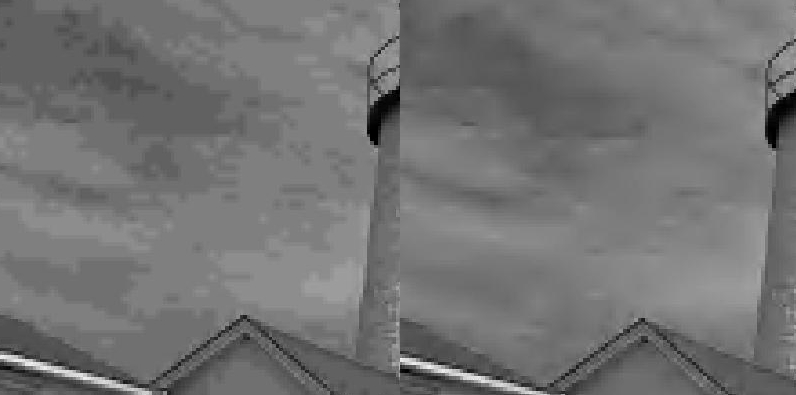
\includegraphics[width=1.0\linewidth, center]{z_dwt_1_5.jpg}
\captionof{figure}{\small{\textbf{Visual quality between one- and five-iteration DWT on Lighthouse image, using equal MSE scheme.} Using only one iteration gives a more `pixelated' image compared to the one constructed from more iteration.}}
\end{Figure}

\begin{Figure}
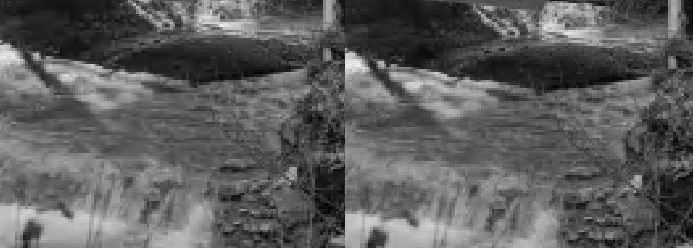
\includegraphics[width=1.0\linewidth, center]{mse_const.jpg}
\captionof{figure}{\small{\textbf{Visual quality between between equal MSE and constant quantiser.} There is hardly any differences between the two schemes, even after zooming into the images.}}
\end{Figure}
\end{multicols}

\small
\begin{center}
\begin{tabular}{|l|l|p{7cm}|}
\hline
\textbf{Energy Compaction Scheme} & \textbf{Optimal Compress Ratio} & \textbf{Artefacts \& Key Details} \\
\hline
\textit{Pyramid} & 1.3301 & Pixelated images. Reduced with increased depth of pyramid.\\
\hline
\textit{Dicrete Cosine Transform} & 3.0566 & Block artefacts, which enhances with increase transform size. \\
\hline
\textit{Lapped Bi-orthogonal Transform} & 3.3539 & Block artefacts from DCT suppressed, but ringing effect and `ghost' objects appear when the transform size is large. \\
\hline
\textit{Discrete Wavelet Transform} & 3.1023 & Pixelated at low number of iterations, which is suppressed when more is performed. \\
\hline
\end{tabular}
\captionof{table}{\textbf{Comparison between different energy compaction schemes}. These results are specific to Lighthouse picture only.}
\end{center}

\end{document}
